% !TeX root = ../main.tex
\section{Assortativität}
\label{sec:assortativitaet}

Kapitel~\ref{sec:zusammenhalt} hat gezeigt, dass sich Athleten wiederholt
treffen. Nun fragen wir, wer sich trifft. Verbinden sich Athleten bevorzugt
mit ähnlichen Athleten? Wir untersuchen die Assortativität nach Nation,
Geschlecht, Jahrgang, Leistung und Degree im Arbeitsnetz. Für kategorische
Attribute berechnen wir sie über die Mixing Matrix, für numerische als
Pearson-Korrelation der Werte an beiden Enden jeder Kante. Als Leistung
dient wie in Kapitel~\ref{sec:zentralitaet} der maximale FINA-Punktewert.

\subsection{Gesamtnetz}
Für Nation, Geschlecht, Jahrgang und Leistung prüfen wir die
Nullhypothese, dass das Attribut nicht mit den Kanten zusammenhängt. Dazu
verteilen wir die Werte 10\,000-mal zufällig auf die Athleten, die
Netzwerkstruktur bleibt wie in Kapitel~\ref{sec:reduktion} unverändert. Der
Degree entsteht aus dem Netz selbst. Für ihn vergleichen wir deshalb mit
den 100 Referenz-Netzwerken des bipartiten Configuration Model aus
Kapitel~\ref{sec:zusammenhalt}. Das Signifikanzniveau beträgt
$\alpha = 0{,}05$ mit Holm-Korrektur über die fünf Tests.

\begin{table}[H]
  \centering
  \caption{Assortativität im Arbeitsnetz. Referenz für Nation, Geschlecht,
  Jahrgang und Leistung sind 10\,000 Permutationen der Attribute, für den
  Degree 100 Referenz-Netzwerke des bipartiten Configuration Model. Eigene
  Auswertung.}
  \label{tab:assortativitaet}
  \begin{tabular}{@{}lrrrr@{}}
    \toprule
    Attribut & $r$ & Referenz Mittel & Referenz Maximum & $p$ \\
    \midrule
    Jahrgang & 0,85 & 0,00 & 0,01 & $< 0{,}0001$ \\
    Nation & 0,42 & 0,00 & 0,00 & $< 0{,}0001$ \\
    Degree & 0,40 & 0,12 & 0,16 & $< 0{,}01$ \\
    Leistung & 0,37 & 0,00 & 0,01 & $< 0{,}0001$ \\
    Geschlecht & 0,04 & 0,00 & 0,01 & $< 0{,}0001$ \\
    \bottomrule
  \end{tabular}
\end{table}

Alle Attribute sind signifikant assortativ (Tabelle~\ref{tab:assortativitaet}),
auch nach Holm-Korrektur. Am stärksten verbinden sich Athleten gleichen
Jahrgangs, danach folgen Nation, Degree und Leistung. Das Geschlecht ist
mit $r = 0{,}04$ vernachlässigbar, wie schon in Kapitel~\ref{sec:reduktion}.
Auch die Degree-Assortativität geht klar über das bipartite Configuration
Model hinaus. Athleten mit vielen Kontakten treffen sich also häufiger
untereinander, als die Projektion allein erklärt. Das passt zu
Kapitel~\ref{sec:zusammenhalt}, wo internationale Meisterschaften das Netz
zusammenhalten. In Kapitel~\ref{sec:reduktion} hatten wir für die Nation
eine Korrelation von 0,25 berechnet. Sie bezog sich auf alle
Athletenpaare, die Assortativität dagegen nur auf die Kanten. Beide messen
dieselbe Tendenz, nur anders normiert. Die Rangvarianten bestätigen die
Werte, Ausreisser treiben sie also nicht.

Der Jahrgang ist der stärkste Befund. Verbundene Athleten unterscheiden sich
im Median um drei Jahre, zufällige Paare um neun
(Abbildung~\ref{fig:jahrgang}). Fast die Hälfte der verbundenen Paare liegt
höchstens zwei Jahre auseinander, bei zufälligen Paaren ist es ein Sechstel.
Das erklärt die Generationen-Communities aus Kapitel~\ref{sec:communities}.

\begin{figure}[H]
  \centering
  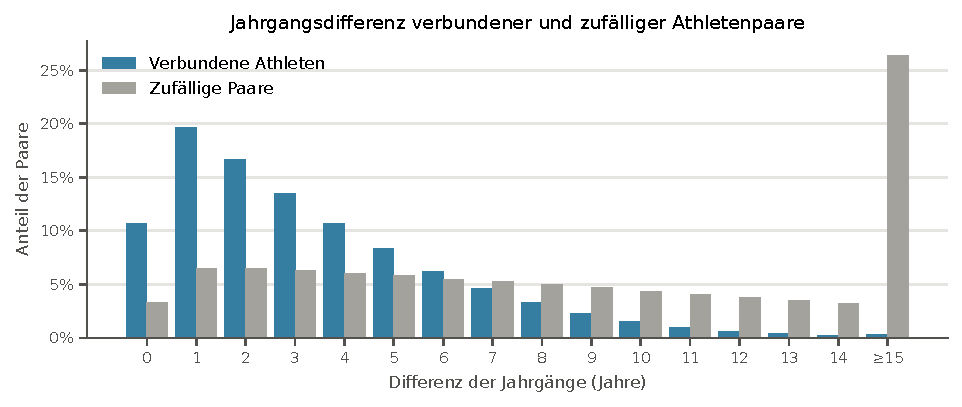
\includegraphics[width=\textwidth]{08_jahrgang.pdf}
  \caption{Differenz der Jahrgänge für verbundene Athleten (blau) und gleich
  viele zufällige Paare mit bekanntem Jahrgang (grau). Die letzte Klasse
  fasst Differenzen ab 15 Jahren zusammen. Eigene Auswertung.}
  \label{fig:jahrgang}
\end{figure}

\subsection{Elite-Club oder Altersklassen}
Ein globaler Wert kann lokale Muster verdecken. Abbildung~\ref{fig:lokal}
zeigt die Assortativität nach Leistung und Jahrgang deshalb getrennt für
die Generationen und die elf nationalen Communities aus
Kapitel~\ref{sec:communities}. Für die nationalen Communities zentrieren
wir die Werte vorher je Community. Sonst würden die unterschiedlichen
Leistungsniveaus der Nationen eine Assortativität vortäuschen.

\begin{figure}[H]
  \centering
  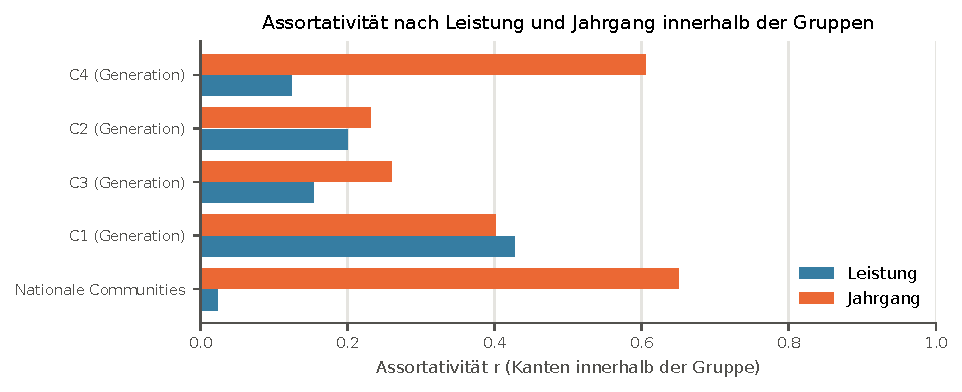
\includegraphics[width=\textwidth]{08_lokal.pdf}
  \caption{Assortativität nach Leistung (blau) und Jahrgang (orange) für
  Kanten innerhalb der Generationen und der elf nationalen Communities. Für
  die nationalen Communities sind die Werte je Community zentriert. Eigene
  Auswertung.}
  \label{fig:lokal}
\end{figure}

Die Muster unterscheiden sich deutlich. In der jüngsten Generation C1
treffen sich starke Schwimmer bevorzugt mit starken ($r = 0{,}43$). In den
älteren Generationen ist dieser Effekt schwächer (0,12 bis 0,20). Innerhalb
der nationalen Communities fehlt er fast ganz ($r = 0{,}02$, jede einzelne
zwischen $-0{,}01$ und 0,05), dafür prägt dort der Jahrgang besonders stark
($r = 0{,}65$). National treffen sich also Gleichaltrige unabhängig von
ihrem Niveau, etwa an Meisterschaften mit Altersklassen. Einen Elite-Club,
in dem sich Starke mit Starken treffen, gibt es erst international und vor
allem in der aktuellen Generation. Kapitel~\ref{sec:zentralitaet} hat
gezeigt, dass stärkere Schwimmer zentraler sind. Hier zeigt sich, wo sie
sich treffen.

Die Leistungsassortativität bleibt fast gleich, wenn wir vom Punktewert den
Mittelwert desselben Jahrgangs abziehen ($r = 0{,}36$) oder den Mittelwert
desselben Jahrs der besten Leistung ($r = 0{,}35$). Sie entsteht also
nicht nur dadurch, dass verbundene Athleten gleich alt sind oder ihre
Bestleistung in derselben Saison erzielten, deren Punkte durch
Punktetabellen oder Hightech-Anzüge ähnlich verschoben sind.

Die Werte beschreiben Zusammenhänge und keine Ursachen. Da die
TOP100-Auswahl eine eher homogene Leistungselite abbildet, unterschätzen
sie die Leistungsassortativität wahrscheinlich eher. Für die älteste Generation C4 ist
zudem die dünnere Datenlage aus Kapitel~\ref{sec:zusammenhalt} zu
berücksichtigen.
